\chapter{Introduction}\label{chap:introduction}
http://www.laneas.com/sites/default/files/publications/1/PachosEtAl2016Misconceptions.pdf
network congestion client server
client->server Content Delivery Networks (CDNs) caching

Replicate popular contents in many geographical areas
save bandwidth on the network path by avoiding unncesessary multiphop retranmissions.
REPHRASE. As a byproduct, it also decreases access time (latency) by decreasing the distance between the two communicating entities.

Today eport of Cisco [1] predicts a massive increase of Internet devices connected through the wireless
access
steep increase in mobile traffic which is expected to reach by 2018
oughly 60\% of total network traffic, the majority of which will be video.

5G wireless networks with higher access rates
with increased densification of network infrastructure on the other.

he explosion of access rates
and number of base stations, the backhaul of wireless networks will also become congested motivates further the use of caching: store popular reusable information at the base
stations to reduce the load at the backhaul

The research community suggests to
n the network of the future, memory units can be installed in gateway routers between
the wireless network and the Internet (e.g. in 4G this is called S-GW), in base stations of different
sizes (small or regular size cells), and in end-user devices

fog computing


In the remainder of this chapter we provide an overview over the scientific contributions of this monograph in \refsec{sec:introduction:scientific_contribution} and provides an outline of this monograph in \refsec{sec:introduction:outline}.

%\section{Scope of Considered Stakeholders}\label{sec:introduction:considered_stakeholders}


\section{Scientific Contribution}\label{sec:introduction:scientific_contribution}

\begin{figure}
\centering
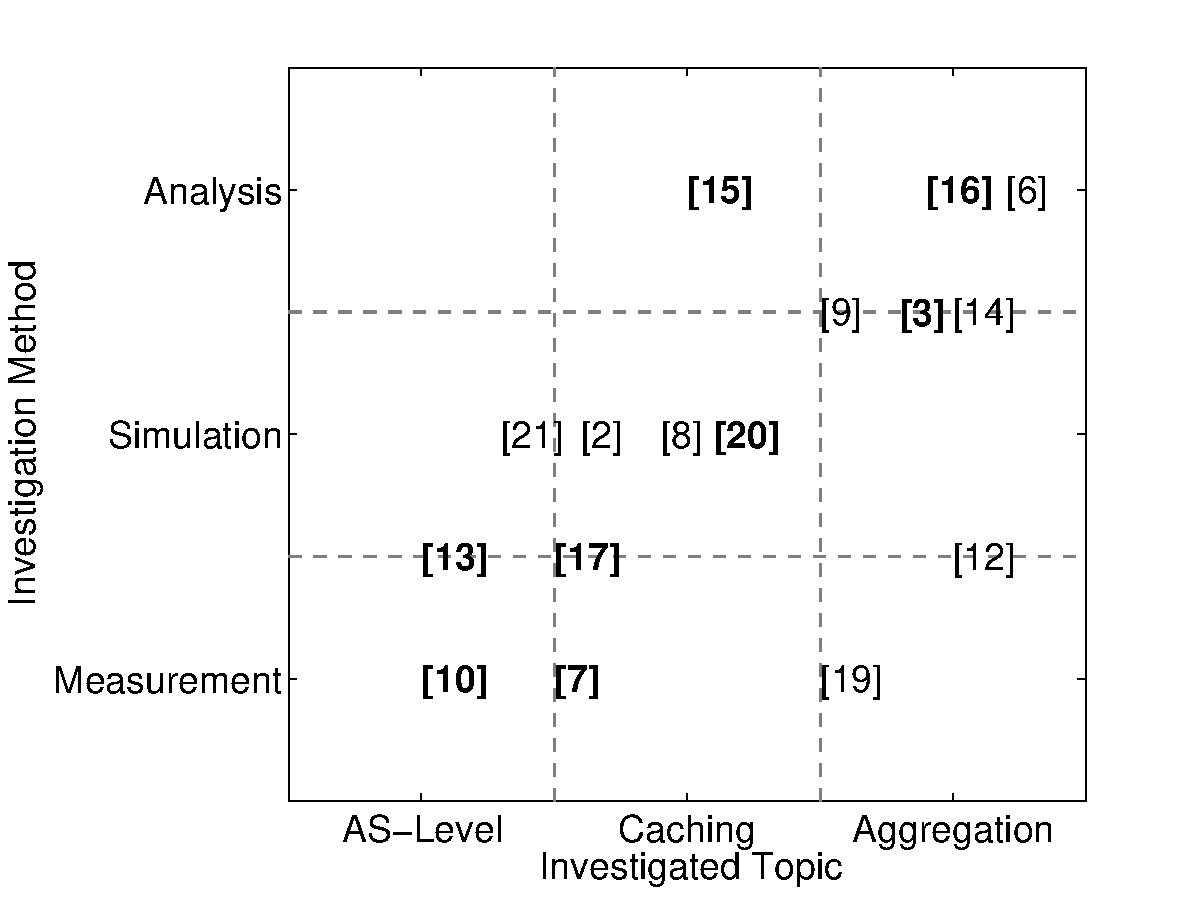
\includegraphics{figures/publications}
\caption{Contribution of this work as a classification of the research studies conducted by the author.}\label{fig:introduction:publications}
\end{figure}

In \reffig{fig:introduction:publications} we classify the areas of research as well as scientific methods used in relation to the chapters of this monograph.
The x-axis shows the impacted areas of research, i.e. topics related to the mobile network, the application domain or cloud technologies.
The y-axis details the applied scientific method.
In the theoretical area methods from queueing theory, mean value analysis and the analysis of random variables are used.
Measurements were performed using testbeds and custom software tools.
Simulation studies, performed using \gls{DES}, and created analysis tools are summarised in the practical area.

Annotations are used to highlight scientific publication whose content contributes to the respective chapters.

The first contribution of this monograph is a discussion of the impact of
We study the impact of , and investigate the potential of network parameter optimisation as a means to .

As a second contribution, we provide models for
We show that the streaming mechanism allows
However, further study shows that in fact
Furthermore, we provide
TODO REPHRASE: During off-peak operation of the network, the users can cheaply populate their caches with parts of popular contents.

As a third contribution, we discuss the
To this end, we study the performance of
We derive guidelines for
Furthermore, we discuss a mechanism to
Finally, we present a mechanism to

\section{Outline of Thesis}\label{sec:introduction:outline}

In \refchap{chap:aslevel} we study
First,
Then,
Finally,

\refchap{chap:hierarchical} focuses on
For Video Streaming, we study the impact
To address the second scenario, we discuss

In \refchap{chap:aggregation} we study
First,
Then,
We analyse traffic characteristics and use them as input for a simulation model
Combining these results, we evaluate the impact of different virtual server configurations and scaling strategies.
Finally, we consider resource allocation

In \refchap{chap:conclusion} we provide a summary of the major contributions of this work and suggest future potential research directions.
